\documentclass{beamer}
\usepackage{etex}
\usepackage[utf8]{inputenc}
\usepackage[T2A]{fontenc}
\usepackage{graphics,graphicx,epsfig}
\usepackage{amssymb,amsfonts,amsthm,amsmath,mathtext,cite,enumerate,float}
\usepackage[english,russian]{babel}
\usepackage[all]{xy}
\usepackage{pgf}
\usepackage[debug,outputdir={docgraphs/}]{dot2texi}
\usepackage{tikz}
\usepackage{scalefnt}
\usepackage{graphicx}
\usepackage{ulem}\normalem
\usetheme{Warsaw}
\usecolortheme{sidebartab}
\usefonttheme[onlylarge]{structurebold}
\setbeamerfont*{frametitle}{size=\normalsize,series=\bfseries}
\setbeamertemplate{navigation symbols}{}
\setbeameroption{show notes}
\setbeamertemplate{itemize items}[circle]
\setbeamertemplate{enumerate items}[circle]
\setbeamertemplate{blocks}[rounded][shadow=false]

\newtheorem{algo}{Алгоритм}
\newtheorem{stat}{Утверждение}
\newtheorem{defin}{Определение}
\newtheorem{theo}{Теорема}

\newcommand{\NBin}[1]{\mathbf{NBin}\ \text{#1}\ }
\newcommand{\NUn}[1]{\mathbf{NUn}\ \text{#1}\ }
\newcommand{\LVar}{\mathbf{LVar}\ }
\newcommand{\LC}{\mathbf{LC}\ }

\begin{document}

\title[Порождение и выбор моделей\hspace{4em}\insertframenumber/\inserttotalframenumber]{Алгоритмы индуктивного порождения и критерии выбора оптимальной существенно нелинейной регрессионной модели для аппроксимации измеряемых данных}
\author{Г. И. Рудой}
\institute{Московский физико-технический институт \vfill
Факультет управления и прикладной математики \vfill
Кафедра интеллектуальных систем \vfill
Научный руководитель: В. В. Стрижов}
\date{Июнь 2014}

\begin{frame}
  \maketitle
\end{frame}

\begin{frame}{Цель работы}
  \begin{itemize}
	\item Формулирование и обоснование понятия устойчивости моделей:
	\begin{itemize}
	  \item Критерий выбора моделей.
	  \item Исследование погрешности в измеряемых данных.
	\end{itemize}
  \end{itemize}
\end{frame}

\begin{frame}{Постановка задачи исследования устойчивости}
  Дано:
  \begin{itemize}
   \item Обучающая выборка $D$:
     \[
	   D = \{ \mathbf{x}_i, y_i \} \mid i \in \{ 1, \dots, \ell \}.
     \]
   \item Семейство $\mathcal{F}$ параметрических функций $f = f(\mathbf{x}, \boldsymbol{\omega})$.
   \item Функционал качества $S$:
     \[
       S = S (f (\cdot, \boldsymbol{\omega}), D) \mid f \in \mathcal{F}, \quad S \rightarrow \mathop{\min}\limits_{\boldsymbol{\omega}}
     \]
  \end{itemize}
  
  Требуется:
  \begin{itemize}
    \item Исследовать зависимость $\hat{\boldsymbol{\omega}} = \mathop{\arg \min}\limits_{\boldsymbol{\omega}} S$ от вариации $D$.
    \item Проверить возможность экспертного применения $f$ при данной вариации $D$.
  \end{itemize}
\end{frame}

\begin{frame}{Известные результаты}
  \begin{itemize}
    \item Случай линейной регрессии:
      \[
        y_i = ax_i + b + \xi_i \mid i \in \{ 1, \dots, n \}.
      \]
    \item Верхние границы ошибок в SVM [Vapnik2000].
    \item Малые изменения входных данных в сетях глубокого обучения [Szegedy2014].
  \end{itemize}
\end{frame}

\begin{frame}{Предлагаемый алгоритм}
  \begin{enumerate}
    \item Фиксируется параметрическая модель $f \in \mathcal{F}$:
      \[
        f = f(\mathbf{x}, \boldsymbol{\omega}) \in \mathcal{F}.
      \]
    \item Начальный оптимальный вектор параметров:
      \[
        \hat{\boldsymbol{\omega}}_f(D) = \mathop{\arg \min}\limits_{\boldsymbol{\omega}_f} S(f, D).
      \]
  \end{enumerate}
\end{frame}

\begin{frame}{Предлагаемый алгоритм}
  \begin{enumerate}
    \setcounter{enumi}{2}
    \item Варьируется выборка:
      \[
        \acute{D}(\Sigma^{\mathbf{x}}, \boldsymbol{\sigma}^y) = \{ \mathbf{x}_i + \boldsymbol{\xi}^{\mathbf{x}}_i, y_i + \xi^y_i \mid i \in 1, \dots, \ell \}.
      \]
    \item Оптимальный вектор параметров для варьированной выборки $\acute{D}$:
      \[
    		\hat{\boldsymbol{\omega}}_f (\acute{D} (\Sigma^{\mathbf{x}}, \boldsymbol{\sigma}_y)) = \mathop{\arg \min}\limits_{\boldsymbol{\omega}_f} S (f (\cdot, \boldsymbol{\omega}_f), \acute{D} (\Sigma^{\mathbf{x}}, \boldsymbol{\sigma}_y)).
      \]
    \item Разность с начальным оптимальным вектором $\hat{\boldsymbol{\omega}}_f$:
      \[
        \Delta\hat{\boldsymbol{\omega}}_f(\acute{D} (\Sigma^{\mathbf{x}}, \boldsymbol{\sigma}_y) ) = \hat{\boldsymbol{\omega}}_f(D) - \hat{\boldsymbol{\omega}}_f (\acute{D} (\Sigma^{\mathbf{x}}, \boldsymbol{\sigma}_y))
      \]
   \end{enumerate}
\end{frame}

\begin{frame}{Предлагаемый алгоритм}
  \begin{enumerate}
    \setcounter{enumi}{5}
    \item Шаги 3-5 повторяются $N$ раз:
      \[
        \acute{\mathcal{D}}_N (\Sigma^{\mathbf{x}}, \boldsymbol{\sigma}_y) = \{ \acute{D}_1 (\Sigma^{\mathbf{x}}, \boldsymbol{\sigma}_y), \dots, \acute{D}_N (\Sigma^{\mathbf{x}}, \boldsymbol{\sigma}_y) \}.
      \]
    \item Вычисляется стандартное отклонение каждой компоненты вектора параметров:
      \[
        \sigma_{\omega_i} = \text{stddev} ((\Delta\hat{\boldsymbol{\omega}}_f)_i).
      \]
    \item Устойчивость $i$-го параметра относительно компоненты $j$ описания:
      \[
        T^N_f(i, j, \Sigma^{\mathbf{x}}, \boldsymbol{\sigma}_y) = \frac{\frac{\sigma_{\omega_i}}{\hat{\omega}_i}}{r(\{\frac{\boldsymbol{\sigma}^\mathbf{x}_{k j}}{\mathbf{x}_{k j}}\}_{k = 1}^{\ell})}.
      \]
  \end{enumerate}
  
  $r$ выбирается экспертом:
  \begin{itemize}
    \item $r(a_1, \dots) = a_1$~--- случай равенства относительных погрешностей.
    \item $r(a_1, a_2, \dots, a_{\ell}) = \frac{\sum_{i = 1}^{\ell} a_i}{\ell}$~--- средняя относительная погрешность.
  \end{itemize}
\end{frame}

\begin{frame}{Случай независимых коэффициентов}
  \begin{theo}[Рудой]
    Пусть стандартные отклонения $j$-ых компонент $\mathbf{x}$ одинаковы:
    \[
      \forall i_1, i_2, j: \sigma_{i_1 j}^{\mathbf{x}} = \sigma_{i_2 j}^{\mathbf{x}}.
    \]
    Пусть коэффициенты $\omega_i$ попарно не коррелируют:
    \[
      \forall i_1, i_2: \text{Cov} (\omega_{i_1}, \omega_{i_2}) = 0.
    \]
    Тогда для достаточно малых $\sigma_{ij}^\mathbf{x}$:
    \begin{align*}
      \{ \sigma_{\omega_i} (\boldsymbol{\sigma}_{\cdot 1}, \boldsymbol{\sigma}_{\cdot 2}, \dots, \boldsymbol{\sigma}_{\cdot |\mathbf{x}|}) \}^2 &=
        \{ \sigma_{\omega_i} (\boldsymbol{\sigma}_{\cdot 1}, 0, 0, \dots, 0) \}^2 + \nonumber \\
        & + \{ \sigma_{\omega_i} (0, \boldsymbol{\sigma}_{\cdot 2}, 0, \dots, 0) \}^2 + \nonumber \\
        & + \dots + \nonumber \\
        & + \{ \sigma_{\omega_i} (0, 0, \dots, 0, \boldsymbol{\sigma}_{\cdot |\mathbf{x}|} \}^2.
      \label{eq:pypha_variance}
    \end{align*}
  \end{theo}
\end{frame}

\begin{frame}{Вычислительный эксперимент: дисперсия полимеров}
  Дано:
  \begin{itemize}
    \item $D_j = (\lambda_i^j, n_i^j) \mid i \in \{ 1, \dots, 17 \}, j \in \{ 1, 2 \}.$
    \item Экспертные предположения.
  \end{itemize}
  
  Требуется:
  \begin{itemize}
    \item $n_j = n_j(\lambda).$
    \item Оценить адекватность $n_1 (\lambda) - n_2 (\lambda)$.
  \end{itemize}
\end{frame}

\begin{frame}{Алгоритм порождения моделей}
  \[
    Q_f = \frac{1}{1 + S_f} \left(\alpha + \frac{1 - \alpha}{1 + \text{exp} (\frac{C(f)}{\beta} - \tau)}\right).
  \]
  \begin{itemize}
    \item $\alpha$~--- влияние штрафа за сложность, $0 \ll \alpha < 1$,
    \item $\beta > 0$~--- строгость штрафа за сложность,
    \item $\tau$~--- желаемая сложность модели.
  \end{itemize}

  \begin{figure}[h]
    \vspace{-20pt}
    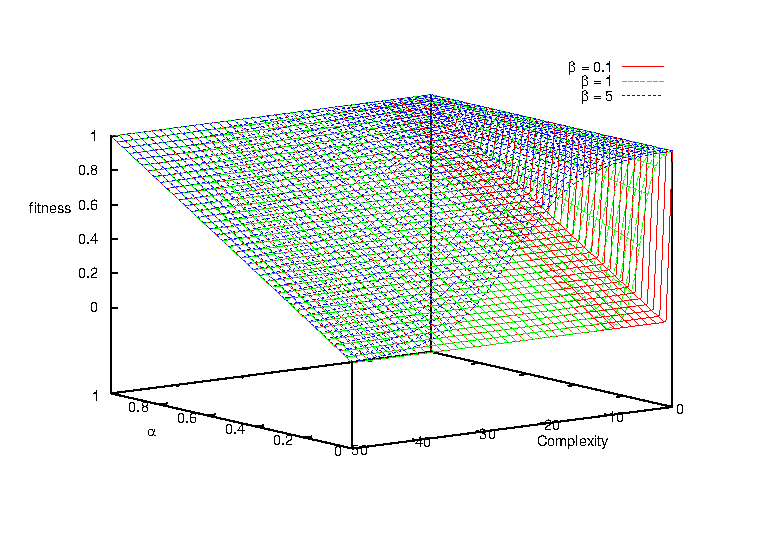
\includegraphics[scale=0.5]{figs/fitness.eps}
    \vspace{-30pt}
  \end{figure}
\end{frame}

\begin{frame}{Порожденные модели}
  Две модели:
  \begin{itemize}
    \item $n_1(\lambda) = 1.34 + \frac{3.54 \cdot 10^3}{\lambda^2} + \frac{2 \cdot 10^3}{\lambda^4}$.
    \item $n_2(\lambda) = 1.34 + \frac{11.6}{\lambda} + \frac{17.37}{\lambda^2} + \frac{0.0866}{\lambda^3} + \frac{2.95 \cdot 10^{-4}}{\lambda^4} + \frac{8.54 \cdot 10^{-7}}{\lambda^5}.$
  \end{itemize}
  
  \begin{table}[h]
    \centering
    \begin{tabular}{| c | c | c | l | c | c | c |} \hline
  	$\tau$	& Суперпозиция		& $MSE$					& $C(f)$		& $Q(f)$ \\ \hline
	10	  	& $n_1$		  		& $2.4 \cdot 10^{-8}$	& 13			& 0.095	\\ \hline
	30		& $n_2$				& $3.9 \cdot 10^{-9}$	& 31			& 0.031	\\ \hline
    \end{tabular}
  \end{table}
\end{frame}

\begin{frame}{Устойчивость моделей}
\begin{table}[h]
    \centering
    \begin{tabular}{c | c}
	  $n_1$ & $n_2$ \\ \hline
	  \includegraphics[scale=0.4]{{figs/even/p1.txt_coeff0.dat}.eps} & \includegraphics[scale=0.4]{{figs/all/p1.txt_coeff0.dat}.eps} \\
    \end{tabular}
    \caption{Графики стандартного отклонения первого коэффициента для моделей $n_1$ и $n_2$.}
  \end{table}
\end{frame}

\begin{frame}{Устойчивость моделей}
\begin{table}[h]
    \centering
    \begin{tabular}{l | c c c}
	  $n$ & $\omega_1$ & $\omega_2$ & $\omega_3$ \\ \hline
	  1 & \includegraphics[scale=0.25]{{figs/even/p1.txt_coeff0.dat}.eps} & 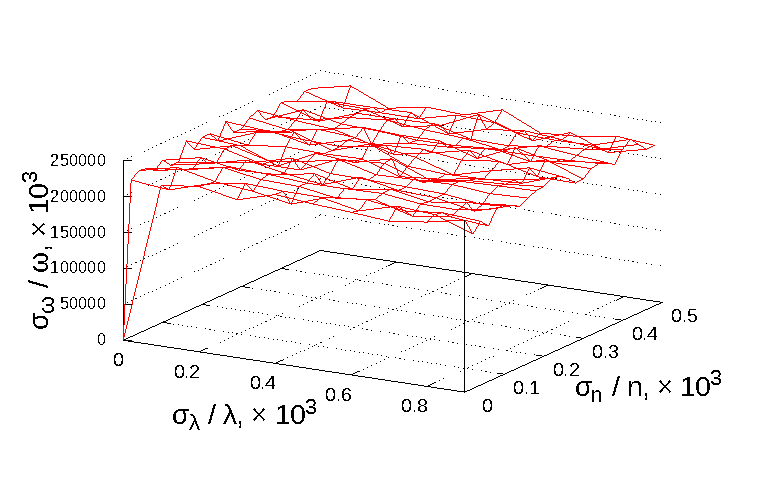
\includegraphics[scale=0.25]{{figs/even/p1.txt_coeff1.dat}.eps} & 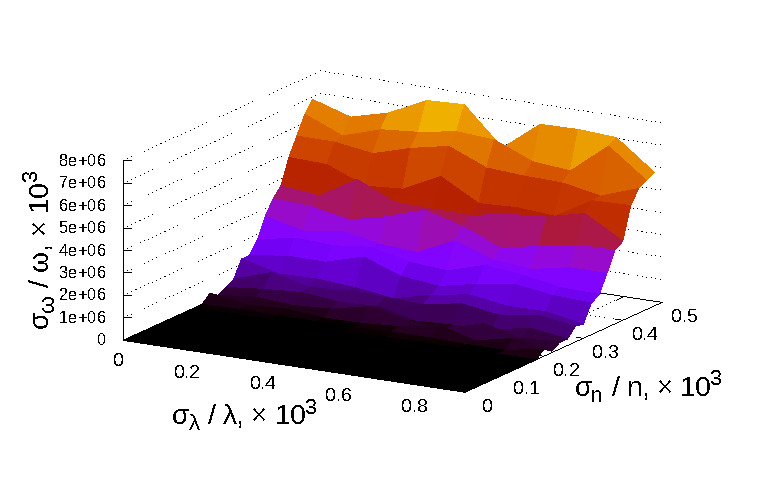
\includegraphics[scale=0.25]{{figs/even/p1.txt_coeff2.dat}.eps} \\
	  2 & 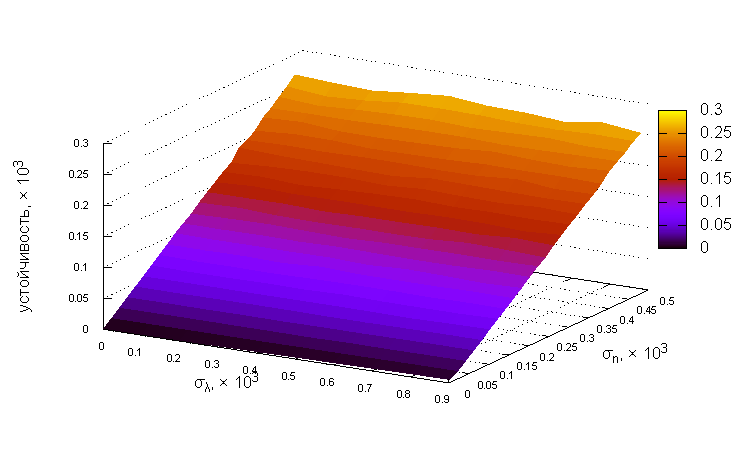
\includegraphics[scale=0.25]{{figs/all/p2.txt_coeff0.dat}.eps} & 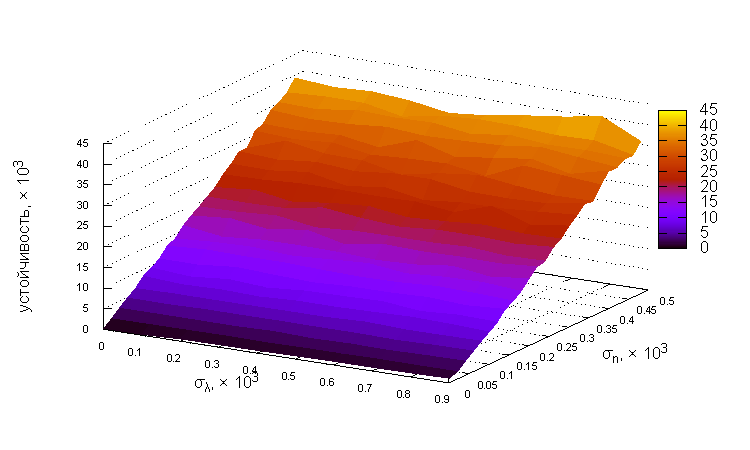
\includegraphics[scale=0.25]{{figs/all/p2.txt_coeff1.dat}.eps} & 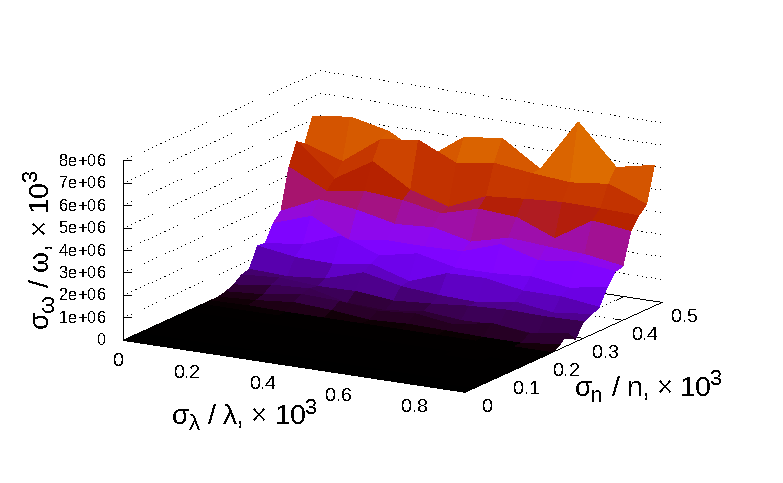
\includegraphics[scale=0.25]{{figs/all/p2.txt_coeff2.dat}.eps}
    \end{tabular}
    \caption{Графики стандартного отклонения первых трех коэффициентов для моделей $n_1$ и $n_2$.}
  \end{table}
\end{frame}

\begin{frame}{Разделяемость моделей}
  \begin{table}[h]
    \centering
    \footnotesize
    \begin{tabular}{| l | c | c | c | c |} \hline
  	Полимер		& $\omega_1$		& $\omega_2$		& $\omega_3$		& MSE	\\ \hline
      1			& 1.34946		& 3558.95		& 1924.33		& $2.2 \cdot 10^{-8}$		\\ \hline
      2			& 1.34047		& 3118.84		& 1578.59		& $1.4 \cdot 10^{-8}$		\\ \hline
  	Разность	& $6.71 \cdot 10^{-3}$	& $1.41 \cdot 10^{-1}$	& $2.2 \cdot 10^{-1}$	&	\\ \hline
    \end{tabular}
    \caption{Значения коэффициентов для модели $n_1$ и их относительная разность.}
  \end{table}
  
  \begin{table}[h]
    \centering
    \footnotesize
    \begin{tabular}{| l | c | c | c |} \hline
	  Коэфф.	& $(2 \cdot 10^{-4}; 2 \cdot 10^{-5})$	& $ (6 \cdot 10^{-4}; 6 \cdot 10^{-5}) $	& $ (9 \cdot 10^{-4}; 2 \cdot 10^{-4}) $ \\ \hline
	  1		& $1.22 \cdot 10^{-5}$					& $ 3.59 \cdot 10^{-5} $					& $ 1.19 \cdot 10^{-4} $		\\ \hline
	  2		& $1.48 \cdot 10^{-3}$					& $ 4.38 \cdot 10^{-3} $					& $ 1.44 \cdot 10^{-2} $		\\ \hline
    \end{tabular}
    \caption{Значения стандартного отклонения для коэффициентов модели $n_1$ для первого полимера в зависимости от относительных дисперсий $(\frac{\sigma_{\lambda}}{\lambda}, \frac{\sigma_n}{n})$.}
  \end{table}
\end{frame}

\begin{frame}{Лагранжева интерполяция}
  \[
    L(x) = \prod_{i = 0}^\ell y_i \prod_{j = 0, j \neq i}^\ell \frac{x - x_j}{x_i - x_j},
  \]
  \begin{figure}[h]
    \centering
    \includegraphics[scale=0.7]{{figs/lagrange/p1.txt_coeff0.dat}.eps}
    \caption{Поверхность стандартного отклонения коэффициента $\omega_0$.}
    \label{fig:lagrange_i_0}
  \end{figure}
\end{frame}

\begin{frame}{Публикации и работы}
  \begin{itemize}
    \item Анализ устойчивости существенно нелинейных регрессионных моделей к погрешностям в измеряемых данных~--- <<ЖВММФ>> (направлено в журнал).
    \item О возможности применения методов Монте-Карло в анализе нелинейных регрессионных моделей~--- <<СибЖВМ>> (направлено в журнал).
    \item Доклад на <<Труды МФТИ>> 2013.
    \item Доклад на <<Ломоносов>> 2014.
  \end{itemize}
\end{frame}

\begin{frame}{Результаты}
  \begin{itemize}
    \item Предложено понятие устойчивости параметров модели.
    \item Обосновано использование понятия устойчивости параметров модели в качестве критерия выбора моделей.
    \item Продемонстрировано использование понятия устойчивости для анализа применимости экспертных моделей.
    \item Исследованы различные регрессионные модели и связь предложенного критерия с критериями ошибки и сложности модели.
  \end{itemize}
\end{frame}

\end{document}